%for a more compact document, add the option openany to avoid
%starting all chapters on odd numbered pages
\documentclass[12pt]{cmuthesis}

% This is a template for a CMU thesis.  It is 18 pages without any content :-)
% The source for this is pulled from a variety of sources and people.
% Here's a partial list of people who may or may have not contributed:
%
%        bnoble   = Brian Noble
%        caruana  = Rich Caruana
%        colohan  = Chris Colohan
%        jab      = Justin Boyan
%        josullvn = Joseph O'Sullivan
%        jrs      = Jonathan Shewchuk
%        kosak    = Corey Kosak
%        mjz      = Matt Zekauskas (mattz@cs)
%        pdinda   = Peter Dinda
%        pfr      = Patrick Riley
%        dkoes = David Koes (me)

% My main contribution is putting everything into a single class files and small
% template since I prefer this to some complicated sprawling directory tree with
% makefiles.

% some useful packages
\usepackage{times}
\usepackage{fullpage}
\usepackage{graphicx}
\usepackage{amsmath}
\usepackage{cite}
\usepackage{multirow}
\usepackage[numbers,sort]{natbib}
\usepackage[pageanchor=true,plainpages=false, pdfpagelabels, bookmarks,bookmarksnumbered,
%pdfborder=0 0 0,  %removes outlines around hyper links in online display
]{hyperref}
\usepackage{setspace}
\usepackage{subfigure}
\usepackage{titlesec}
\DeclareMathOperator*{\argmin}{arg\,min}
\newcommand\addtag{\refstepcounter{equation}\tag{\theequation}}
\titleformat{\chapter}[hang] 
{\normalfont\LARGE\bfseries}{\chaptertitlename\ \thechapter:}{1em}{}

% Approximately 1" margins, more space on binding side
%\usepackage[letterpaper,twoside,vscale=.8,hscale=.75,nomarginpar]{geometry}
%for general printing (not binding)
\usepackage[letterpaper,twoside,vscale=.8,hscale=.75,nomarginpar,hmarginratio=1:1]{geometry}

% Provides a draft mark at the top of the document. 
\draftstamp{\today}{DRAFT}

\begin {document} 
\frontmatter

%initialize page style, so contents come out right (see bot) -mjz
\pagestyle{empty}

\title{ %% {\it \huge Thesis Proposal}\\
{\bf Inharmonicity Regression against Pitch for Automatic Guitar Tablature Transcription}}
\author{Jonathan Michelson}
\date{May 2017}
\Year{2017}
\trnumber{}

\committee{
Dr. Richard Stern, Dr. Thomas Sullivan \\
}

\support{}
\disclaimer{}

% copyright notice generated automatically from Year and author.
% permission added if \permission{} given.

%\keywords{Stuff, More Stuff}

\maketitle

%\begin{dedication}
%For my dog
%\end{dedication}

\pagestyle{plain} % for toc, was empty

%% Obviously, it's probably a good idea to break the various sections of your thesis
%% into different files and input them into this file...

%\doublespacing
\begin{abstract}
We present an additional method for automatic tablature transcription of clean monophonic guitar audio, extending work done by Barbancho in 2012 \cite{barbanchoi2012}. First, for each string, we regress note pitches against their inharmonicity estimates. Then we use these learned linear regressions to predict unseen guitar notes; the system classifies a pitch's string label as the one whose regression approximates the note's inharmonicity with minimal error. Given the tuning of the guitar that produced the unseen note, we infer its associated tablature, which allows for further string classification refinement by rejecting and reassigning implausible fret assignments. The highest F-scores achieved with this system were: (numbers.) We also derive and evaluate an inharmonicity adjustment factor to allow for transcription of arbitrarily-tuned guitars, provided the tuning is known. We find, surprisingly, that our system's transcription performance on alternate-tuning guitars is constant regardless of this inharmonicity adjustment.

\end{abstract}
%\singlespacing

%\begin{acknowledgments}
%My advisor is cool.
%\end{acknowledgments}



\tableofcontents
%\listoffigures
%\listoftables

\mainmatter

%% Double space document for easy review:
%\renewcommand{\baselinestretch}{1.66}\normalsize

% The other requirements Catherine has:
%
%  - avoid large margins.  She wants the thesis to use fewer pages, 
%    especially if it requires colour printing.
%
%  - The thesis should be formatted for double-sided printing.  This
%    means that all chapters, acknowledgements, table of contents, etc.
%    should start on odd numbered (right facing) pages.
%
%  - You need to use the department standard tech report title page.  I
%    have tried to ensure that the title page here conforms to this
%    standard.
%
%  - Use a nice serif font, such as Times Roman.  Sans serif looks bad.
%
% Other than that, just make it look good...
\noindent
\chapter{Introduction} 
\section{Guitar and Tablature} The guitar is a popular musical instrument whose family comprises a diverse collection of stringed instruments. Its most prominent classes are the acoustic, classical, and electric guitars, and intraclass variation in characteristics such as body shape, string material, and amplification mode is high. Despite this diversity, the majority of guitar configurations have six strings tuned to $E2$ ($82$Hz), $A2$ ($110$Hz), $D3$ ($147$Hz), $G3$ ($196$Hz), $B3$ ($247$Hz), and $E4$ ($330$Hz). To play, a performer presses these strings with one hand against the neck's metal frets, each of which increase the string's pitch by one half-step, while strumming or plucking them with the other hand. Guitars typically have upwards of 20 frets, allowing for versatile musical passage realizations along the fretboard.

A consequence of this is liberal pitch overlap between neighboring strings. Conventional music scores that represent passages as notes and chords therefore fail to communicate fretboard position. This ambiguity renders scores unfit for guitar students trying to learn more skillful placement of scales and arpeggios, or for enthusiasts trying to decrypt the fretboard positions used on recordings of a virtuosic player's riffs.

Tablature, on the other hand, is an alternative music notation that doesn't suffer from the one-to-many mapping of scores. The staff, instead of representing pitch as in classical scores, depicts a birds-eye view of the guitar neck from the performer's perspective. (see figure). Each of the six horizontal lines signify a corresponding string on the guitar, and numbers on each line specify the fret to be played. Time progresses from left to right as in scores.

Tablature (tabs for short) is widely popular for a number of likely reasons. Its accessibility and intuition is attractive to those without formal musical training; learning from a pictorial representation of one's instrument must seem more attractive to beginners than learning musical theory foundations and decoding scores. And because tabs are easily encodable and interpretable with simple ASCII characters (see figure?), their creation isn't limited to those with knowledge of any sort of tab-specific generation program, unlike with scores.~\cite{macrae2006}.

Accurate tablature transcription is a fairly tedious task, however. Dependable tabs containing few errors typically require a seasoned musician's careful listening to an audio recording, and possibly video recordings if available too. Reliable automation of this transcription task would benefit the guitar student community by expediting quality tab generation and unearthing fretboard positions of guitar riffs in songs for which accurate tabs don't yet exist. Recent technologies proposed to encourage proliferation of tab transcription systems, such as open-source framework ROBOTABA \cite{burlet}, demonstrate a desire among MIR researchers to see this theoretically mature but practically nascent field mature into student-benefitting applications. Closely related to tab transcription is the task of string classification: producing the correct tablature is straightforward if the guitar's tuning is known and the correct string labels are identified. In the next chapter, we present much of the work that's been done in these fields.

\section{Inharmonicity} Inharmonicity seems to be a key feature in successful string discrimination systems. Due to the -------- ~\cite{fletcher1998}, a vibrating string's harmonic partials are skewed upward in frequency according to: 
\[
f_k = kf_{0}\sqrt{1+\beta k^2} \addtag
\]
where $f_k$ is the $k$th harmonic of fundamental $f_0$ and $\beta$ is the string's inharmonicity, defined by
\[
\beta = \frac{\pi Q d^4}{64 T l^2}. \addtag
\]
In words, the inharmonicity $\beta$ of a vibrating string is dimensionless quantity that depends on the string's Young's modulus $Q$, diameter $d$, tension $T$, and vibrating length $l$, and scales the degree of deviation of the string's $k$th partial according to equation 2.1. Note that for an ideally harmonic string, $\beta = 0$ and (2.1) reduces to $f_k = kf_0$, aligning with intuition about harmonics' ideal locations in frequency as simply integer multiples of the fundamental.

This phenomenon is audible in lower pitch registers because of the necessity of thicker longer strings, and is therefore important for increased realism of synthesized instrument sounds~\cite{jarvalainen2003,fletcher}. Interestingly, not critically audible for acoustic guitar sounds though~\cite{karjalainen}. 

Inharmonicity's suitability for the string discrimination task can be understood through equation (2.2). The six strings of any guitar necessarily exhibit different combinations of $Q$, $d$, and $T$ due to varying thicknesses, material, and tuning. Thus each string has an "inharmonic signature" which presumably distinguishes it from the others. As $l$ varies along the neck when different frets are selected, these "inharmonic signatures" reduce to coefficients on a 2nd-order polynomial that relates inharmonicity to vibration length $l$. In other words, it's reasonable to expect each string's inharmonicity to vary with length $l$ (or equivalently, pitch $P$) in a revealing manner according to its string's unique "inharmonic signature". (Figure). This phenomenon has been exploited by some previous work to obtain favorable string classification results.



\noindent
\chapter{Literature Review}
\section{Inharmonicity Estimation}
Explicit estimation of inharmonicity was first attempted by Galembo in 1979 and 1986~\cite{galembo}. Several additional methods for automated estimation have been proposed in the last two decades. Galembo et al.~\cite{galembo1994} hypothesized a connection between partials-based fundamental pitch estimates and the degree of inharmonicity in a spectrum. They specifically investigated cepstral analysis and a variant of the harmonic product spectrum method applied to both synthetic tones and recorded piano notes. They found that, because these two techniques leverage periodicity in the frequency domain to produce their pitch estimates, inharmonicity influenced the quality of the estimates in a deterministic manner.
 
 The same authors in~\cite{galembo1999} introduced another method in 1999, dubbed the inharmonic comb filter (ICF) method. 

Rauhala~\cite{rauhala} introduced an efficient procedure in 2007 that iteratively catalogued estimates of the partial frequencies' deviations and returns increasingly better estimates of the inharmonicity. The algorithm is initialized with a reasonable first estimate of inharmonicity, and then the note's spectrum is searched for partial peaks. Differences are measured between the locations of these discovered peaks and those of the expected peaks, according to equation (X.X.X), and the aggregate deviation trend is used to refine the inharmonicity estimate -- a majority of positive differences implies the inharmonicity should be reduced, and a majority of negative differences implies the opposite.

In 2009, Hodgkinson~\cite{hodgkinson} proposed a yet more efficient and accurate algorithm. exploiting median-adjustive-trajectories (MAT's) of consecutive partials' deviations, and incorporates refinements such as Complex Spectrum ------- to further improve accuracy and efficiency of the inharmonicity estimate.

\section{Automatic Tablature Generation}
A subtle distinction should be drawn between methods that focus on tablature generation versus tablature transcription. In the former task, the goal is generally production of a plausible tablature which is optimal in some sense (mechanical difficulty for the performer, spatial difficulty, etc.), whereas in the latter, the goal is exact recovery of the original tablature. These objectives are abstractly similar but notably different in practice.

Tablature generation has seen lots of work. Gagnon -- NNs for hand position. Godsill -- Bayesian modelling of inharmonic signals. Radisavljevic -- Viterbi solution through graph. radicioni -- graph search. Tuohy -- genetic algorithm. Yazawa -- multipitch estimation, dynamic programming for graph search. Burlet -- Deep Belief Network.

\section{Automatic Tablature Transcription}
The tablature transcription task is also well studied. Ogrady -- hexaphonic pickup.
In Barbancho et al. ~\cite{barbancho2009}, the authors attempt guitar string classification using features such as nontonal spectrum, etc., but achieve discouraging results.
Barbancho et al. ~\cite{barbanchoi2012}
Estimation typically involves searching a note's spectrum for peaks in the vicinity of multiples of the fundamental, then cataloguing located peaks' deviations from their ideal locations, and fitting a polynomial -- one of whose coefficients corresponds to a good estimate of the inharmonicity -- to the deviations curve. Barbancho~\cite{barbanchoi2012} achieves good tablature transcription using open-strings' inharmonicities and checking unknown notes' inharmonicities against those of string candidates. In various supervised classification approaches~\cite{abesser2012, kehling2014, dittmar2013}, the authors achieve good string transcription after training on standard-tuning guitar audio and using inharmonicity as one of their features.

\noindent
\chapter{Inharmonicity Regression against Pitch}
\section{Motivation}
This work exploits inharmonicity's deterministic variation with respect to fret positions along a given string. Barbancho~\cite{barbanchoi2012} showed that the inharmonicity $\beta(s,n)$ of a note produced by string $s$ at fret number $n$ could be expressed in terms of the inharmonicity of the open-string note $\beta(s,0)$ according to:
\[
\beta(s,n) = \beta(s,0)2^{\frac{n}{6}} \addtag
\]
In other words, the variation in inharmonicity along a given string is restricted to the trajectory defined by the function in $n$ above. We can think of this trajectory as a characterization of the inharmonic quality of the string. If we combine this result with the reasonable expectation that each guitar string $s\in\{1,2,3,4,5,6\}$, due to its mechanical and physical differences from its neighbors, will produce a distinguishable open-string note inharmonicity $\beta(s,0)$, it follows that an unlabeled note played on the same guitar could be mapped to its originator string simply by (1) computing its inharmonicity and (2) assigning it to the string whose pre-computed inharmonicity variation track most closely approximates it. This method could conceivably be extended to unlabeled notes from unseen guitars if the $\beta(s,0)$ used were determined to be reliably typical of most guitar strings. 

Thus, the research questions to address in the assessment of this method are the quality of the inharmonicity estimate and, in the case where the unlabeled note is from a different guitar, the compatibility of the unidentified guitar's $\beta(s,0)$'s with those of the known guitar.

Regression seems to be a natural tool for implementation of this method, as it could find the weights that best characteri

\section{String Classification}
We collect all notes with common string labels in our training data, and we perform linear regression of their inharmonicities $\beta$ against their fundamental pitches $m$ (in MIDI note number format). We do this for each string label. Let $s \in \{1,2,3,4,5,6\}$ be the string label to which each training note is assigned, and $N_s$ be the number of notes we have belonging to string label $s$. If we let $\mathbf{x}_s^{(i)} = 1 + m_s^{(i)}$ represent the $i$th note with fundamental pitch $m^{(i)}$ belonging to string $s$ , and $\beta_s^{(i)}$ be the inharmonicity of the $i$th note belonging to string $s$, we can solve
\[
\mathbf{w}_s = \argmin_{\mathbf{w}}{\sum_{i=1}^{N_s}{(\beta^{(i)}_s - \mathbf{w}^T\mathbf{x}^{(i)}_s)^2}}\addtag
\]
which yields the weight vector $\mathbf{w}_s$ that minimizes the sum of squared error between the measured and predicted inharmonicities of the notes belonging to string $s$. Now that we've learned a quantification of each strings' inharmonic quality, we can use this to predict unseen notes.

For prediction, we take the $n$th note in our test set, characterized by tuple $(m^{(n)},\beta^{(n)})$ where $m^{(n)}$ is its MIDI pitch number and $\beta^{(n)}$ is its inharmonicity. We'd like to transform this into another tuple $(s^{(n)},f^{(n)})$ corresponding to the appropriate string and fret to which this unknown note should be assigned. A straightforward solution is to assign to $s^{(n)}$ the index $j$ of the regression weights $\mathbf{w}_j$ whose predicted inharmonicity $\hat\beta_j$ approximates the measured inharmonicity $\beta^{(n)}$ with least error. More formally, we solve 
\[
s = \argmin_{j}{(\beta^{(n)} - \hat{\beta}_{j})^2} \addtag
\]
where $\hat\beta_j$ is the inharmonicity prediction of string $j$ according to its learned regression, given by
\[
\hat{\beta}_{j} = \mathbf{w}_{j}^T\mathbf{x}^{(n)} \addtag
\]
where, as before, $\mathbf{x}^{(n)} = 1 + m^{(n)}$. 

\section{Tablature Conversion and Refinement}
To generate tablature, we still need to infer notes' fret positions. This is a trivial task provided we know the tuning $\mathbf{t} = [m_1, m_2, m_3, m_4, m_5, m_6]^T$ of the unknown guitar, where $m_s$ is the MIDI pitch number of the open note on string $s$. Because we already have an estimate of the $n$th unknown note's MIDI pitch $m^{(n)}$, simply taking the difference between $m^{(n)}$ and its assigned string's open pitch $m_s$ yields the fret on which the note was played; each fret on a guitar increases the string's pitch by one half-step ,or equivalently the MIDI pitch number by one integer.

The merit of this fret assignment routine is dependent on the string assignment. If an incorrect string is assigned to note $n$, the fret assignment will be consistent with the string but necessarily incorrect as well. In some cases, an incorrect string assignment could yield a negative fret assignment, which is entirely nonsensical. A simple fix that intuitively fits the proposed regression model is to reassign the string label to that of the regression of next least prediction error. This harmonizes well with the reality that the regressions are only generally predictive, since they're learned from averages of the training data; for the cases in which nonsensical strings are selected, we attribute the error to the deviant behavior of the test note's inharmonicity, and conclude that the next most sensible label reassignment is that of the string whose regression, on average, best explains the test note's inharmonicity. This process can be iterated for as long as fret assignments continue being nonsensical, until all string reassignments are exhausted.

\section{Tuning Compensation}
Though standard tuning is the most common pitch configuration of six-string guitars, there exist numerous other tunings in which performers often play. Aside from altering the musicality of the instrument, alternate tunings complicate the transcription process by introducing uncertainty about the open-string pitches. They distort inharmonicity-based methods, since the tensions $T$ of alternately-tuned guitar strings differ from those in standard-tuned strings, thereby affecting estimation of the inharmonicity. 

Current transcription systems don't address this degree of freedom. Obstacles include the fact that guitar recording datasets usually feature only standard-tuning because of its prominence. The method proposed by Barbancho~\cite{barbanchoi2012} is tuning-invariant, but requires access to recordings of the the test guitar's open strings. Other supervised learning systems~\cite{kehling2014, dittmar2013, abesser2012} are trained and evaluated only on standard-tuning guitars.

A possible approach to augment inharmonicity-based string classifiers with tuning-invariant performance is to simply introduce a scaling factor on the expected inharmonicity. The fundamental frequency $f_0$ of an ideal vibrating string is related to its tension $T$ according to
\[
f_0 = \frac{1}{2L}\sqrt{\frac{T}{\mu}} \addtag
\]
where $L$ is string length and $\mu$ is its density. Solving for $T$, we obtain
\[
T \propto f_0^{2} \addtag
\]
Recognizing that for a change in pitch of $m$ semitones, the equivalent change in frequency is $2^{\frac{m}{12}}$, we see that the proportional change in tension is
\[
T \propto 2^{\frac{m}{6}}f_0^2, \addtag
\]
and that the resulting inharmonicity is therefore
\[
\beta = (2^{-\frac{m}{6}}) \frac{\pi Q d^4}{64 T l^2}. \addtag
\]
If we're given the alternate tuning of the unseen guitar and we have pre-computed inharmonicity regressions of other standard-tuned guitars, we should be able to compensate our predictive regressions by a factor of $2^{-\frac{m}{6}}$ and expect more accurate transcription. This is a straightforward modification for any inharmonicity-exploiting classifier. We report our results with this modification in the next chapter.

\section{Implementation Details}
\subsection{Pre-processing}
Though not in the transcription problem scope, the pre-processing choices we made are worth mentioning to elucidate the specifics and limitations of our method. 

Onset detection was a necessary front-end step. We found that rectified spectral flux with median-filter thresholding~\cite{bello2005,dixon2006} worked well.

For automatic pitch estimation, we resorted to the harmonic sum spectrum~\cite{noll1969}, primarily because of its straightforward implementation. Our method was restricted to monophonic inputs for simplicity, though previous inharmonicity-based transcription systems~\cite{barbanchoi2012,abesser2012,dittmar2013,kehling2014} achieve good performance with polyphony.

\subsection{Inharmonicity Estimation}
We followed the estimation routine used by Barbancho~\cite{barbanchoi2012}, which is similar to that proposed by Rauhala~\cite{rauhala} We summarize Barbancho's algorithm below: 
\begin{enumerate}
\item Estimate a note's fundamental, $\hat{f_0}$.
\item Initialize inharmonicity estimate $\beta = 0$; number of partials to search for at each iteration $K = \{K_1,K_2,K_3,...\}$; and iteration $i=1$
\item Compute $K_i$ expected harmonic locations $f_k$ as integer multiples of the measured fundamental: $f_k = kf_0\sqrt{1+\beta k^2}$, for $k = \{2,3,...K_i\}$.
\item Locate measured partials nearby expected partials
\item Obtain deviations of located partials from their corresponding expected locations. 
\item Fit polynomial $y = ak^3 + bk + c$ to the partials deviations
\item Store $\beta$ estimate as $\frac{2a}{\hat{f_0}+b}$
\item Increment iteration $i = i+1$, then repeat steps 3--7 until list of desired $K$s exhausted.
\end{enumerate}

\noindent
\chapter{Experiments and Results}
We used subsets of the Real World Corpus' Music Instrument Database (RWC-MDB-I)~\cite{goto2003}, subsets of the Fraunhofer Institute for Digital Media Technology's Semantic Music Technologies guitar dataset (IDMT-SMT)~\cite{asdf}, and personal recordings of an electric guitar to conduct our experiments. 

The RWC subset comprises nine guitar recordings (three classical, three acoustic, and three electric), each of which are performed numerous times with varying permutations on certain musicality parameters (playing style, dynamic level, pickup selection). The performances themselves are simply clean, isolated, monophonic enumeration of every fret (from open-string to 12th fret) on every string (from string 6 to string 1), constituting 78 total note plucks per audio file. The resolution is 16 bits per sample, at 44.1kHz. Labels of strings and frets are thus obtained by their location of occurrence in the recording. The classical guitars recorded were a Stafford, a Sakurai Kohno Professional-J, and a Yuichi Imai YJ-II; the three acoustic guitars captured were an Ovation, a Yamaha APX, and Yairi WY1; the electric guitars featured were a Fender Stratocaster, an Aria PE, and an Ibanez Artcore.

The IDMT-SMT guitar dataset focuses on electric guitars, and boasts standardized licks performed across its sample instruments. The bit depth here is 24, with sampling rate equal to 44.1kHz. The subset we used featured six short licks (each between 10 and 30 notes), each of which were captured on three electric guitars: an Aristedes 010, a Fender Stratocaster, and a Gibson Les Paul. Transcriptions which included string and fret labels were saved as accompanying .xml files.

We also recorded a Fender Telecaster at 16 bits and 44.1kHz in the same vein as the RWC database: string and fret enumeration, totaling 78 notes per recording. We captured various tunings: standard, "DADGAD", "WSU" (whole-step up), and "WSD" (whole-step down), and performed each one with a pick and at a similar moderate dynamic level. No other musicality parameters were captured; we focused on tuning variance here.

Table (XX) summarizes the results from our first experiment. We trained linear regressions for each string based on classical (CG), acoustic (AG), and electric (EG) guitar inharmonicities. To evaluate our string classification performance for the CG type, we performed regression on every guitar recording available in the RWC database except for those of CG1, and then made predictions on CG1's recordings and computed its average string-wise F1-scores. We did the same for CG2 and CG3, then string-wise averaged all three guitars' mean F1-scores to obtain the results in Table (XX). The same procedure was followed to obtain the AG and EG string-wise F1-scores. We repeated this experiment another time, learning regressions for only the guitar type which we were evaluating. As expected, string-wise classification performance is superior when regressing on guitar types identical to the test guitar.

F1-scores for RWC recordings
\begin{center}
\begin{tabular} {||c||c|c||c|c||c|c||}
\hline
 & \multicolumn{2}{|c|}{CG} & \multicolumn{2}{|c|}{AG} & \multicolumn{2}{|c|}{EG}\\
\hline
String No. & all & CG & all & AG & all & EG \\
\hline
\hline
1 & 0.39 & $0.25$ & 0.25 & $0.88$ & 0.26 & $0.79$ \\
\hline
2 & 0.26 & $0.47$ & 0.27 & $0.35$ & 0.46 & $0.53$ \\
\hline
3 & 0.12 & 0.65 &  0.12 & 0.67 & 0.07 & 0.10\\
\hline
4 & 0.44 & 0.36 & 0.36 & 0.71 & 0.26 & 0.56\\
\hline
5 & 0.34 & 0.30 & 0.70 & 0.81 & 0.10 & 0.78 \\
\hline
6 & 0.46 & 0.53 & 0.81 & 0.84 & 0.60 & 0.93\\
\hline
\end{tabular}
\end{center}

Next, we learned inharmonicity regressions from almost all standard-tuned RWC electric guitar recordings (and our standard-tuned personal recording), and made predictions on our alternate-tuned personal recordings. We evaluated string-wise F1-score performance both with and without the tuning compensation factor in our system discussed in the previous chapter (XX). Tuning compensation results are denoted by the "comp." column, and original results without compensation are denoted by the "orig." column. See Table (XX).

\begin{center}
F1-scores for one personally recorded electric guitar, at different tuning configurations. 
\begin{tabular} {|c||c||c|c||c|c||c|c|}
\hline
& STANDARD & \multicolumn{2}{|c|}{"DADGAD"} & \multicolumn{2}{|c|}{"WSU"} & \multicolumn{2}{|c|}{"WSD"} \\
\hline
String No. & orig. & orig. & comp. & orig. & comp. & orig. & comp. \\
\hline
1 & 0.96 & 0.70 & 0.70 & 0.96 & 1.00 & 0.67 & 0.78 \\
\hline
2 & 0.73 & 0.32 & 0.32 & 0.89 & 0.96 & 0.35 & 0.52\\
\hline
3 & 0.61 & 0.44 & 0.65 & 0.42 & 0.52 & 0.11 & 0.45\\
\hline
4 & 0.46 & 0.41 & 0.39 & 0.63 & 0.67 & 0.43 & 0.43 \\
\hline
5 & 0.47 & 0.65 & 0.72 & 0.42 & 0.56 & 0.38 & 0.50 \\
\hline
6 & 0.76 & 0.92 & 0.92 & 0.76 & 0.96 & 0.76 & 0.79\\ 
\hline
\end{tabular}
\end{center}

\noindent
\chapter{Conclusions}
\section{}

\begin{figure}[h]
\centering
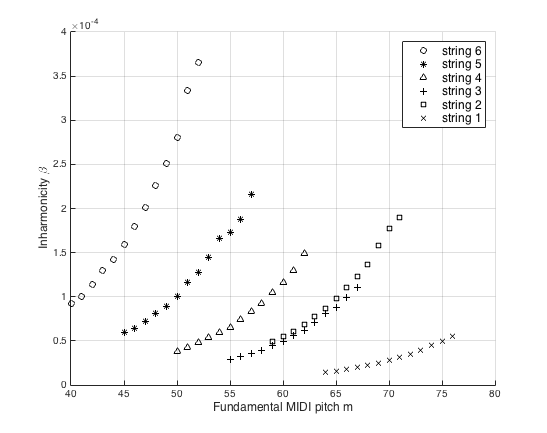
\includegraphics[scale=.6]{beta-v-midi.png}
\caption{Inharmonicities $\beta$ (y-axis) vs. MIDI note number (x-axis). The six different colors correspond to the six string labels E2, A2, D3, G3, B3, E4. This electric guitar recording enumerated the 78 notes between E2 and E5 inclusive in standard-tuning.}
\label{fig:beta}
\end{figure}

\begin{figure}[h]
\centering
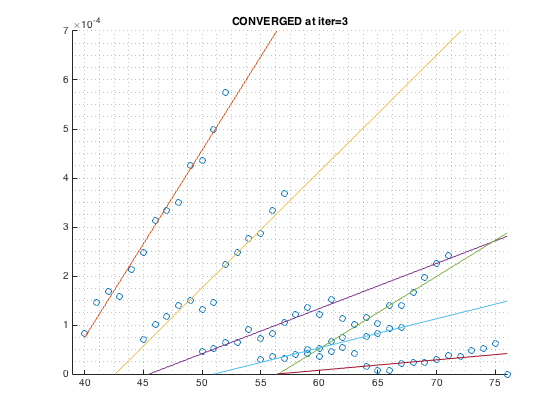
\includegraphics[scale=0.6]{em.png}
\caption{Converged EM estimate of the linear regressions. Same axes as fig. \ref{fig:beta}.}
\label{fig:em}
\end{figure}

%\appendix
%\include{appendix}

\backmatter

%\renewcommand{\baselinestretch}{1.0}\normalsize

% By default \bibsection is \chapter*, but we really want this to show
% up in the table of contents and pdf bookmarks.
\renewcommand{\bibsection}{\chapter{\bibname}}
%\newcommand{\bibpreamble}{This text goes between the ``Bibliography'' header and the actual list of references}
\bibliography{mybib} %your bib file
\bibliographystyle{plainnat}


\end{document}
